\section{Single Page Application Frameworks}
\label{chap:validierung}
Um das Ziel zu erreichen, dass das neue Classroom Response System ohne einen zentralen Server funktionieren kann, muss die Software also komplett clientseitig ausgeführt werden. Es wird also eine Fat-Client-Aufteilung angestrebt.

Für diesen Zweck bietet es sich an, die Software als sogenannte Single Page Application zu implementieren. Das bedeutet, dass die gesamte Anwendung nur eine einzige Webseite lädt. Navigation und dynamische Inhalte werden bei Bedarf asynchron nachgeladen, es wird jedoch keine neue Seite geladen.

Als Framework für die Implementierung der Single Page Application wird das React-Framework ausgewählt. Das Open-Source-Projekt wird von Facebook finanziert und gehört zu den populärsten Frameworks zum Erstellen von Web-Applikationen.

Das React-Ökosystem ist sehr groß und so bietet sich die Erweiterung der App um einige beliebte Muster und Bibliotheken aus der React-Welt an. Das State Management der Anwendung wird im Flux-Pattern in Form der Redux-Bibliothek implementiert.


%
\section{Variable Server-Client-Architektur}
\label{chap:p2p}
Um Unabhängigkeit von einem dedizierten, zentralen Server zu erreichen kann jeder Weclare-Nutzer zum Start einer Sitzung, also zur Laufzeit entscheiden, welche Rolle er in der Topologie einnehmen will (Server oder Client). Unabhängig von der Wahl wird stets der gleiche Code vom Server geladen. Das Programm ist in dieser Hinsicht also vielgestaltig. Im laufenden Fragebetrieb gibt es dann eine fixe Rollenzuteilung unter den Teilnehmern: Der Rechner des Dozent agiert als Server, die Rechner der Studenten sind Clients und somit ergibt sich eine klassische Stern-Topologie.

Es werden also einige Merkmale einer Peer-to-Peer-Architektur erfüllt (die Teilnehmer führen die gleiche Software aus und sind heterogen zusammengesetzt), im strengen Sinne handelt es sich jedoch nicht um eine Peer-to-Peer-Topologie, sondern lediglich um eine variable Form einer Server-Client-Struktur.

Die Entscheidung, dass jeder Teilnehmer variabel entscheiden kann, ob er die Rolle als Server oder Client einnehmen will bedeutet, dass Aspekte wie NAT und der Austausch der IP-Adressen (das Signalling) berücksichtigt werden müssen.

Der Zugriff auf Schnittstellen des Betriebssystems (wie etwa das Netzwerk) durch Browser-Inhalte ist aus Sicherheitsgründen in JavaScript stark eingeschränkt. Die einzige bekannte Möglichkeit, eine omnidirektionale Verbindung zwischen Browsern zu realisieren ist der relativ neue WebRTC-Standard (Abgekürzt für „Web Realtime Communication“).

WebRTC wird hauptsächlich für Echtzeit-Video- und Audio-Anwendungen eingesetzt. Viele Video- und Audiotelefonie-Lösungen (zum Beispiel Skype oder Discord) basieren inzwischen auf dem WebRTC-Protokoll. Neben Audio- und Videoinhalten können aber auch beliebige andere Daten übertragen werden. WebRTC beinhaltet keine Anweisungen für den Austausch der IP-Adressen zwischen beteiligten Parteien. Dieser Teil, das sogenannte Signalling, ist nicht Teil des Standards und muss selbst implementiert werden. Der Aufwand dafür ist relativ hoch, wenn alle gängigen Netzwerk-Situationen berücksichtigt werden sollen. Deswegen wird beim Weclare-Prototyp eine OpenSource-Bibliothek namens PeerJS verwendet, die WebRTC in eine sehr einfache API kapselt und das Signalling-Verfahren beisteuert.

Die mehrfach formulierte Anforderung, keinen dedizierten Server zu benötigen, kann aufgrund des notwendigen Signallings also nicht vollständig erfüllt werden und muss präzisiert werden: Ein dedizierter Server wird lediglich zum Austausch der IP-Adressen der Teilnehmer benötigt. Anwendungsdaten werden nie über einen zentralen Server, sondern immer nur zwischen den Teilnehmern verschickt.
%
\section{Formatierung}
\label{chap:metriken}
Quelltexte können in zwei verschiedenen Kontexten in Fragestellungen auftauchen: Einerseits gibt es unvollständige, kurze Quelltext-Fragmente, die in einen Fließtext eingebunden werden sollen, wie in diesem Beispiel:

\begin{quote}
„Wie viele String-Parameter hat die folgende Java-Methode?\newline
public String m(int i, int s, boolean b) \{ ... \}“
\end{quote}

Dabei handelt es sich nicht um ein syntaktisch nicht vollständiges und nicht-ausführbares Java-Fragment. Um die Lesbarkeit dieses Fragments zu erhöhen, sollte es dennoch optisch deutlich vom Fließtext unterscheidbar sein. Es bietet sich an, den Code in einer Monospace-Schriftart zu formatieren und (wenn möglich) eine syntaktische Einfärbung (Syntax Highlighting) anzuwenden.

Da die Entwicklung einer eigenen Editor-Komponente komplex ist, und es in diesem Bereich bereits eine große Auswahl an Bibliotheken gibt, wird auf eine bestehende Implementierung zurückgegriffen. Dabei müssen folgende Anforderungen von einer solchen Bibliothek erfüllt werden:

\begin{itemize}
    \item \textbf{Integration in React:}  Muss sich leicht in das deklarative React-Framework einbinden lassen.
    \item \textbf{WYSIWYG (What You See Is What You Get):} Der Editor muss stets eine Vorschau aller Formatierungen darstellen, und es soll nicht zwischen einem Markup- und einem Vorschau-Modus gewechselt werden müssen. Formatierungen sollen über Buttons eingefügt werden können.
    \item \textbf{Text-Formatierungen:} Der Editor muss über simple Text-Formatierungen verfügen (zum Beispiel Fettschrift und Kursivierung).
    \item \textbf{Monospace-Schriftart:} Eine Möglichkeit zum Verwenden einer Monospace-Schriftart muss vorhanden sein.
    \item \textbf{Syntax-Highlighting:} Syntaktische, farbliche Hervorhebungen von Code-Fragmenten müssen unterstützt werden (üblicherweise durch ein Plugin/Erweiterung mit einer zusätzlichen Bibliothek wie Highlight.js).
\end{itemize}

Nach dem Erwägen und Ausprobieren diverser Bibliotheken (zum Beispiel Draft.js, Slate, Prosemirror, Quill) fiel die Wahl letztendlich auf den Quill-Editor\footnote{Offizielle Webseite: \url{https://quilljs.com/}}, der alle genannten Anforderungen erfüllt. Quill ist nicht primär für den Einsatz mit React vorgesehen, deswegen wird der Editor in Form der Wrapper-Bibliothek \texttt{react-quill}-Bibliothek\footnote{Offizielle Webseite: \url{https://github.com/zenoamaro/react-quill}} verwendet, die Quill in React-Komponenten bündelt.

\begin{figure}[H]
    \centering
    \setlength{\fboxsep}{0pt}
    \setlength{\fboxrule}{0.5pt}
    \fbox{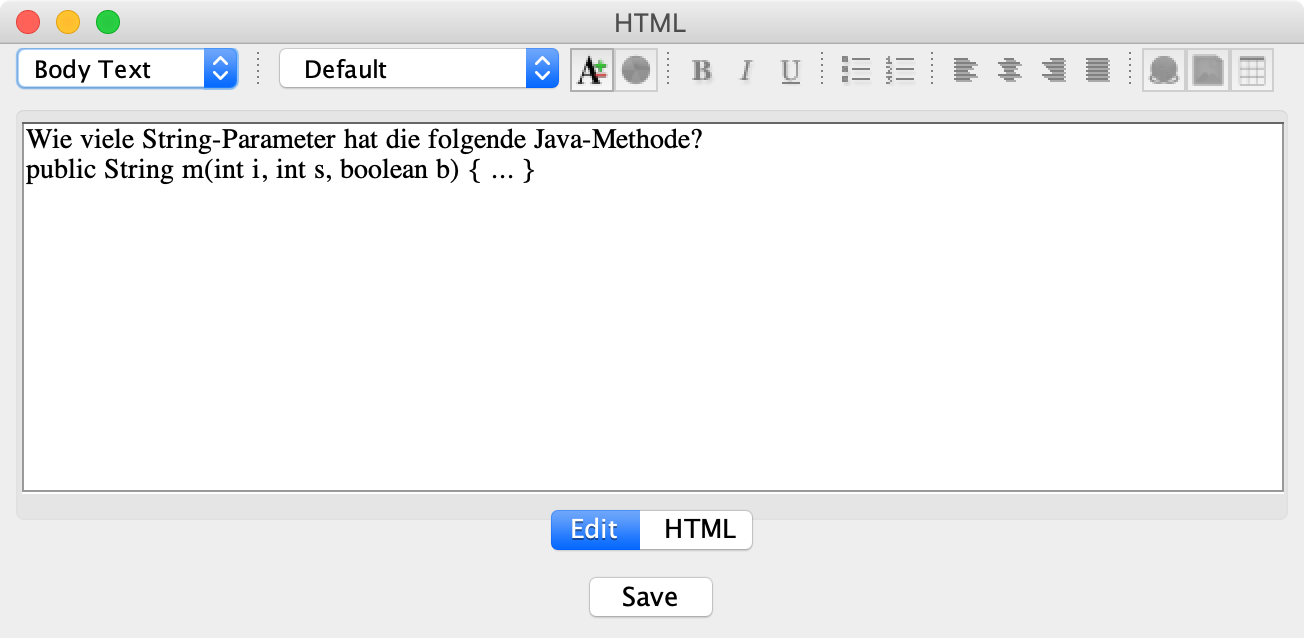
\includegraphics[width=\textwidth-1pt]{chapter/entwurf/bilder/sturesy_editor.png}}
    \caption[StuReSy-Fragen-Editor]{Bearbeiten einer Fragestellung im StuReSy-Fragen-Editor.}
    \label{abb:sturesy_editor}
\end{figure}

\begin{figure}[H]
    \centering
    \setlength{\fboxsep}{0pt}
    \setlength{\fboxrule}{0.5pt}
    \fbox{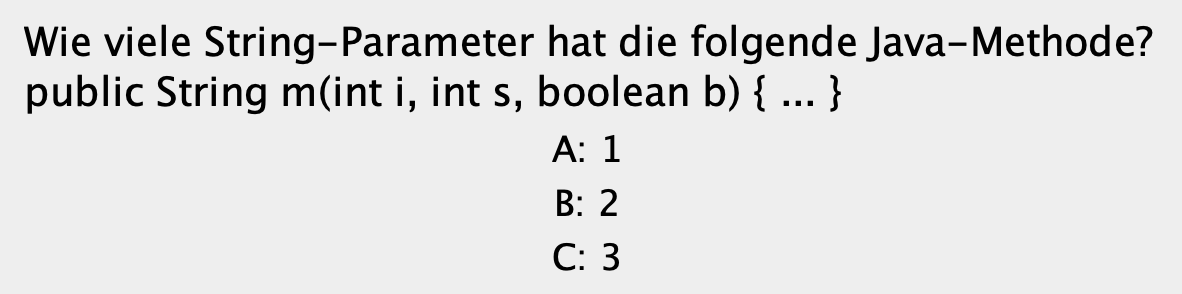
\includegraphics[width=\textwidth-1pt]{chapter/entwurf/bilder/sturesy_fragment.png}}
    \caption[Darstellung eines Code-Fragments in StuReSy]{Darstellung eines Code-Fragments in StuReSy (ohne manuell vorgenommene Formatierungen)}
    \label{abb:sturesy_code_fragment}
\end{figure}


\begin{figure}[H]
    \centering
    \setlength{\fboxsep}{0pt}
    \setlength{\fboxrule}{0.5pt}
    \fbox{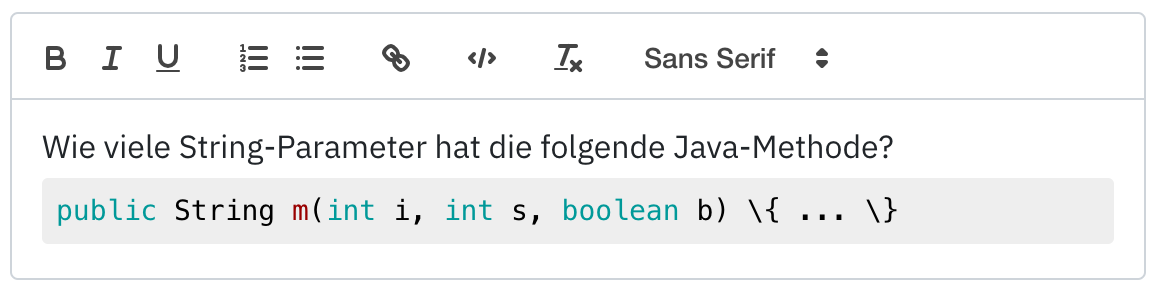
\includegraphics[width=\textwidth-1pt]{chapter/entwurf/bilder/weclare_quill.png}}
    \caption[Quill-Editor von Weclare]{Bearbeiten einer Fragestellung im Quill-Editor von Weclare.}
    \label{abb:weclare_quill}
\end{figure}

\begin{figure}[H]
    \centering
    \setlength{\fboxsep}{0pt}
    \setlength{\fboxrule}{0.5pt}
    \fbox{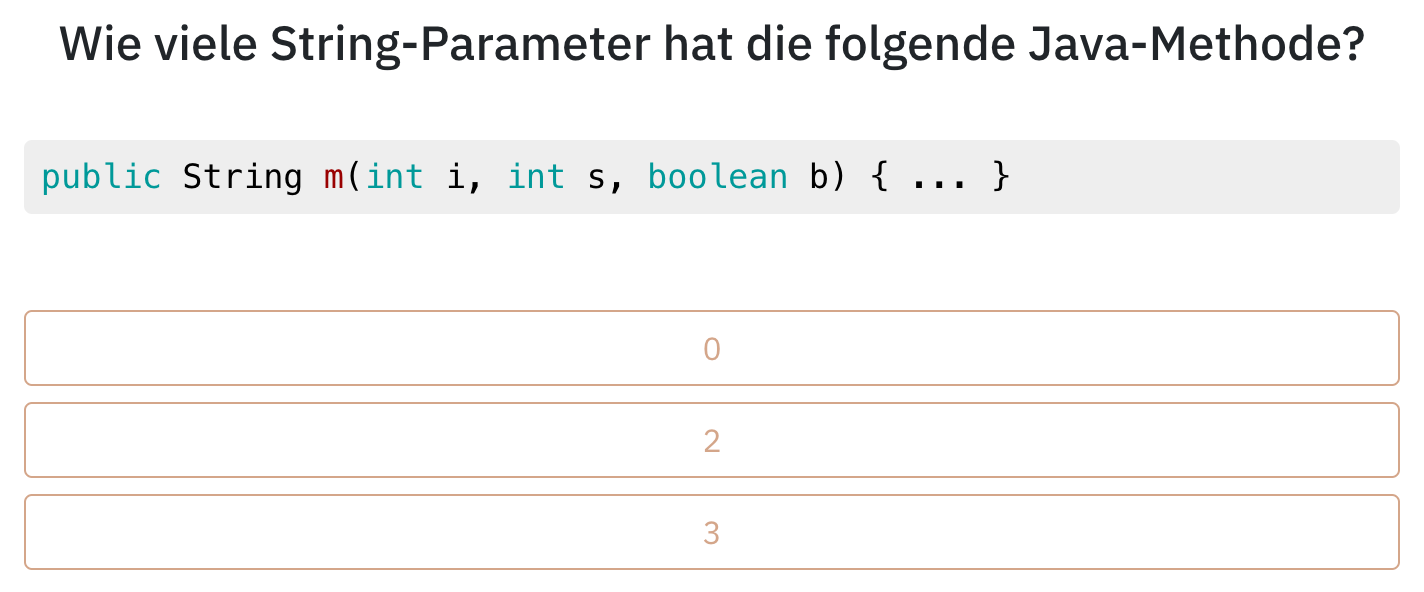
\includegraphics[width=\textwidth-1pt]{chapter/entwurf/bilder/weclare_fragment.png}}%
    \caption[Darstellung eines Code-Fragments in Weclare]{Darstellung eines Code-Fragments in Weclare (Quelltext als Code-Block ausgezeichnet)}
    \label{abb:weclare_code_fragment}
\end{figure}

Der zweite Kontext von Quelltexten in Fragestellungen ist das Einfügen von vollständigem, ausführbarem Code, in Form ganzer Java-Klassen. Solcher Code kann in Weclare direkt im Browser ausgeführt werden. So ein interaktives Code-Beispiel kann allerdings nur einmal pro Frage vorhanden sein und ist auch nicht Teil des Fließtexts. Eine entsprechende Editor-Komponente zum Einfügen solchen Codes sollte also auch funktional darauf zugeschnitten sein: Text-Formatierungen sind nicht mehr notwendig, stattdessen rücken Funktionen wie die korrekte Einrückung von Code-Zeilen und Zeilen-Nummerierungen in den Vordergrund.

Der Quill-Editor kann leider nicht in einem „Code only“-Modus betrieben werden, so dass eine zweite, unabhängige Editor-Komponente für interaktive Code-Abschnitte integriert wird. Mit CodeMirror\footnote{Offizielle Webseite: \url{https://codemirror.net/}} existiert eine sehr beliebte Bibliothek für diesen Zweck, die allerdings auch nicht explizit für den Einsatz im React-Framework bestimmt ist, so dass auch sie in Form einer Wrapper-Bibliothek namens \texttt{react-codemirror2}\footnote{Offizielle Webseite: \url{https://github.com/scniro/react-codemirror2}} zum Einsatz kommt.



\begin{figure}[H]
    \centering
    \setlength{\fboxsep}{0pt}
    \setlength{\fboxrule}{0.5pt}
    \fbox{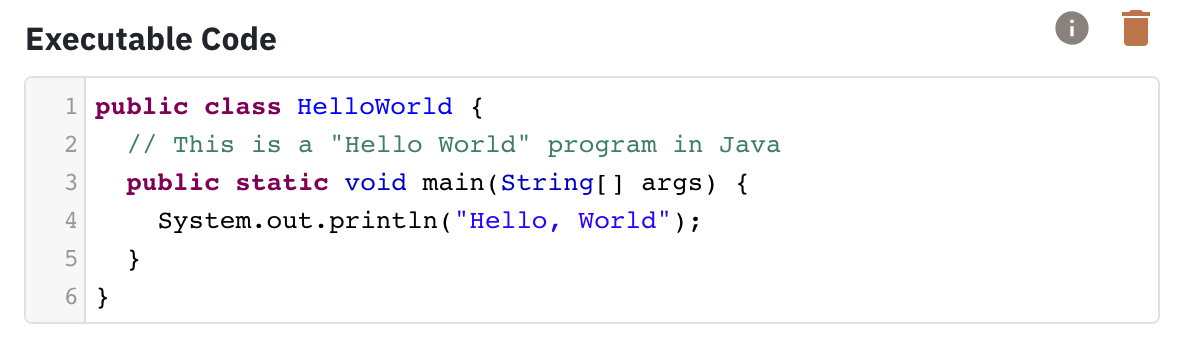
\includegraphics[width=\textwidth-1pt]{chapter/entwurf/bilder/weclare_codemirror.png}}
    \caption[Darstellung eines ausführbaren Java-Quelltexts in Weclare]{Darstellung eines ausführbaren Java-Quelltexts in Weclare mittels der CodeMirror-Bibliothek.}
    \label{abb:weclare_codemirror}
\end{figure}
%
\section{Ausführung}
\label{chap:metriken}
Normalerweise wird Java in einem zweistufigen Prozess ausgeführt. Zunächst wird eine plattformabhängige JVM geladen. Innerhalb dieser JVM wird der Java-Compiler (javac) aufgerufen. Dieser compiliert Java-Quelltext zu Java-Bytecode. Der Java-Bytecode kann dann von der JVM ausgeführt werden. Dieser Ablauf ist in der \ref{abb:java_execution} unter a) dargestellt.

Um Java in einem Browser auszuführen ergeben sich konzeptionell mindestens drei verschiedene Möglichkeiten, die in \ref{Abbildung 4.4} mit den Buchstaben b-d gekennzeichnet sind.

\begin{figure}[H]
    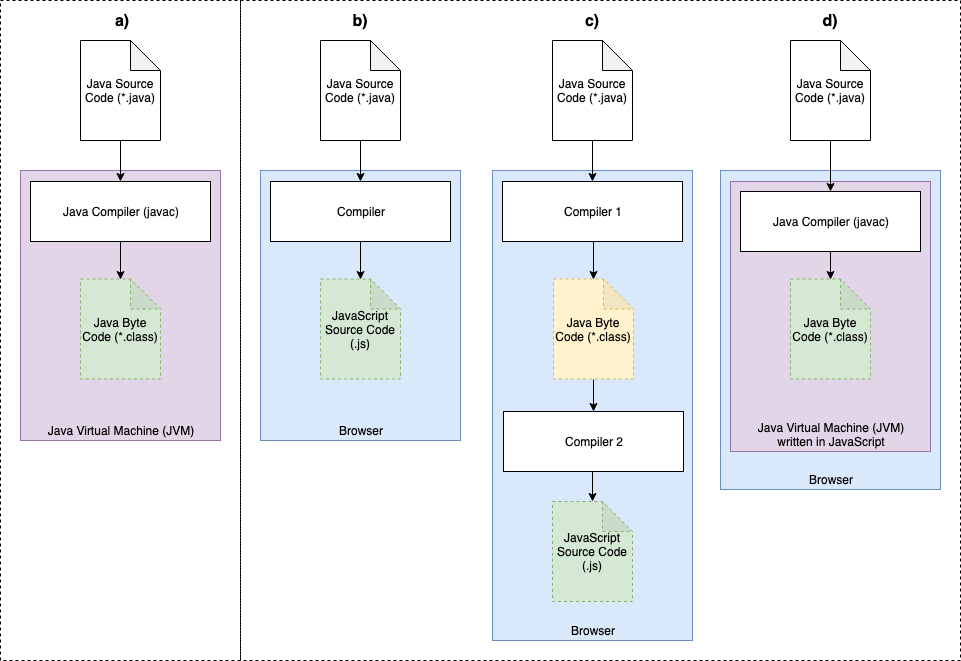
\includegraphics[width=14cm]{chapter/entwurf/bilder/Java_JavaScript_Execution.png}
    \centering
    \caption{Blubb}
    \label{abb:java_execution}
\end{figure}

\begin{itemize}
    \item \textbf{b:} Java-Quelltext wird mit einem Compiler direkt in JavaScript umgewandelt: Diese Variante ist konzeptionell sehr einfach. Zwar gibt es einige Programme, welche Java-Quelltext in JavaScript übersetzen können (zum Beispiel JSweet oder GWT), jedoch sind alle diese Programme entweder in Java selbst oder in anderen Programmiersprachen verfasst. Einen solchen Compiler, der selbst in JavaScript geschrieben wurde, gibt es bisher nicht. Es wäre möglich eines der besagten Programme auf einem separaten Server zu verwenden. Dies würde aber eine weitere Abhängigkeit von einem Server bedeuten, und damit der formulierten Kern-Anforderung widersprechen.
    \item \textbf{c:} Java-Quelltext wird mithilfe eines ersten Compilers in Java-Bytecode übersetzt. Anschließend wird der Java-Bytecode mit einem zweiten Compiler in JavaScript übersetzt. Auch hier ergibt sich das gleiche Problem wie in b). Zwar gibt es Programme, die den jeweiligen Teilschritt übernehmen könnten, jedoch ist keins davon in JavaScript verfasst, so dass es keine Lösung dafür im Browser gibt.
    \item \textbf{d:} Es wird eine JVM verwendet, die in JavaScript implementiert wurde. Mithilfe dieser JVM kann der javac-Compiler geladen werden, um Java-Quelltext in Java-Bytecode zu übersetzen und anschließend auszuführen. Eine solche JavaScript-JVM existiert bereits in Form eines Universitätsprojekt der University of Massachusetts unter dem Namen DoppioJVM. Der konzeptionelle Nachteil dieser Lösung liegt in der benötigten Datenmenge: Um eine komplette JVM im Browser auszuführen wird ebenfalls die Java Runtime Environment benötigt, deren Größe bei etwa 60 Megabyte liegt.
\end{itemize}

In Anbetracht der Tatsache, dass die Ausführung der Code-Beispiele im Browser exakt die gleichen Ergebnisse liefern soll, wie die Ausführung in einer lokalen JVM (zum Beispiel auch in Bezug auf Fehler beim Kompilieren), so ist die Variante d die bevorzugte Lösung und wurde im Rahmen dieser Arbeit in das entstandene CRS integriert.

DoppioJVM ist das Ergebnis der PLASMA-Forschungsgruppe der University of Massachusetts in Amherst, USA. Das Projekt wurde im Jahr 2014 im Rahmen einer wissenschaftlichen Arbeit veröffentlicht und wird von den Autoren selbst wie folgt beschrieben:

\begin{quotation}
„DoppioJVM is a robust prototype Java Virtual Machine (JVM) interpreter
that operates entirely in JavaScript. DoppioJVM implements all
201 bytecode instructions specified in the second edition of the
Java Virtual Machine Specification, supports multithreaded
programs, runs multiple languages that run on top of the JVM, and
implements many of the complex mechanisms and native functionality that JVM programs expect.“
\end{quotation}

Voraussetzung für den Betrieb von DoppioJVM ist ein weiteres Projekt der gleichen Forschungsgruppe: BrowserFS. Dabei handelt es sich um die Implementation eines NodeJS-kompatiblen Dateisystems innerhalb des Browsers. Somit können JavaScript-Programme, die eigentlich für die NodeJS-Laufzeitumgebung gestaltet sind (also Zugriffe auf ein Dateisystem ermöglichen) auch im Browser ausgeführt werden. BrowserFS emuliert ein Dateisystem auf Basis verschiedener Webstandards. So können für den Betrieb der DoppioJVM zum Beispiel die JRE-Komponenten über ein virtuelles Dateisystem bereitgestellt werden, welches auf dem asynchronen Nachladen basiert, oder andere Komponenten der JVM über den LocalStorage des Browsers.

Nachdem das BrowserFS-Dateisystem konfiguriert ist, kann DoppioJVM mit einer relativ einfachen Schnittstelle verwendet werden:

\begin{minipage}{\linewidth}
\begin{lstlisting}
new Doppio.VM.JVM(
  {
    doppioHomePath: "/sys",
    classpath: [".", "/sys/", "/tmp/"]
  },
  (err, jvmObject) => {
    jvmObject.runClass("Loader", [classname], exitCode => {
      if (exitCode !== 0) {
        console.log("JVM exited with an error");
      } else {
        console.log("JVM exited successfully");
      }
    });
  }
);
\end{lstlisting}
\end{minipage}

Die DoppioJVM muss bei jeder Verwendung neu instantiiert werden. Deswegen ist es erforderlich, dass die Kompilierung und Ausführung des gewünschten Java-Codes in einem Aufruf erfolgt. Dazu hat Java einige Möglichkeiten an Bord, die in Form der folgenden Loader-Klasse implementiert wurden:

\begin{minipage}{\linewidth}
\begin{lstlisting}
import javax.tools.*;
import java.lang.reflect.*;
import java.io.*;
import java.net.*;

public class Loader {
  public static void main(String[] args) {
    if (args.length == 0) {
      System.out.println("No class was found.");
      System.exit(1);
    }
    String className = args[0];
    String sourceFile = "/tmp/" + className + ".java";
    String classFile = "/tmp/" + className + ".class";

    System.out.println("Compiling found class '" + className + "'...");

    JavaCompiler compiler = ToolProvider.getSystemJavaCompiler();
    int result = compiler.run(null, null, null, sourceFile, "-d", "/tmp/");

    if (result == 0) {
      try {
        System.out.println("Compilation successful. Executing...");
        System.out.println("---");

        URLClassLoader classLoader = new URLClassLoader(
            new URL[] {new File(classFile).toURI().toURL()}, ClassLoader.getSystemClassLoader());
        Class<?> c = classLoader.loadClass(className);
        Method m = c.getDeclaredMethod("main", String[].class);
        m.invoke(null, new Object[] {});
        classLoader.close();

        System.out.println("Execution successfull");
      } catch (Exception e) {
        e.printStackTrace();
      }
    } else {
      System.out.println("Could not compile");
    }
  }
}
\end{lstlisting}
\end{minipage}

\begin{figure}[H]
    \centering
    \setlength{\fboxsep}{0pt}
    \setlength{\fboxrule}{0.5pt}
    \fbox{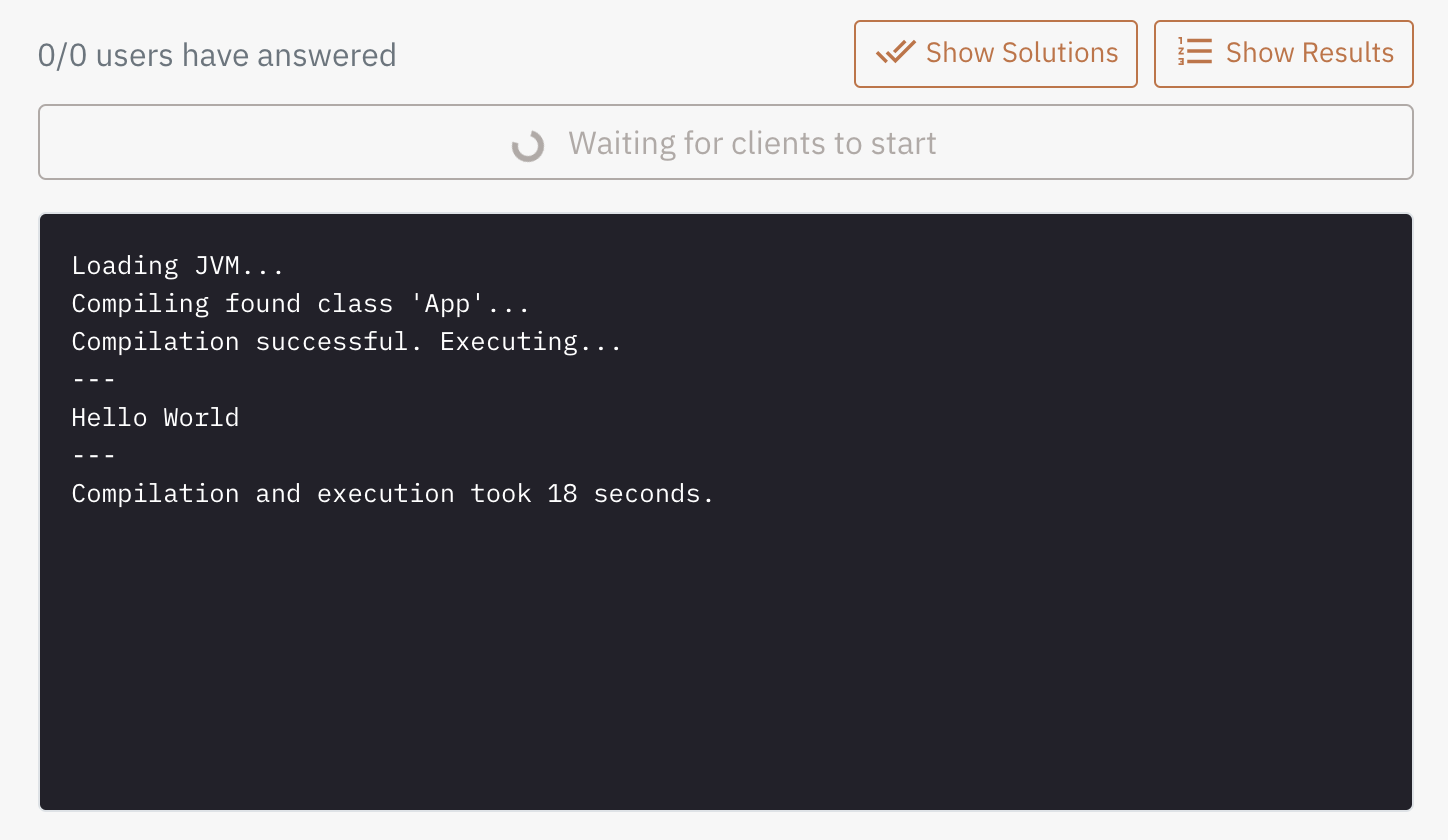
\includegraphics[width=\textwidth-1pt]{chapter/entwurf/bilder/weclare_jvm_console.png}}
    \caption{Ausführung einer Java-Klasse in Weclare mittels DoppioJVM.}
    \label{abb:weclare_jvm_console}
\end{figure}

